\subsection{Systemets Opbygning}

\begin{frame}{Hardware Komponenter}
\begin{columns}
\begin{column}{.48\textwidth}
\begin{description}
\item[Kinect]{Billed-feed til lokalisering}
\item[Robot]{Navigation i og observation af verden}
\item[PC]{Beregning af:}
\begin{itemize}
\item{kort}
\item{robot lokation}
\item{rute}
\end{itemize}
\end{description}
\end{column}
\begin{column}{.48\textwidth}
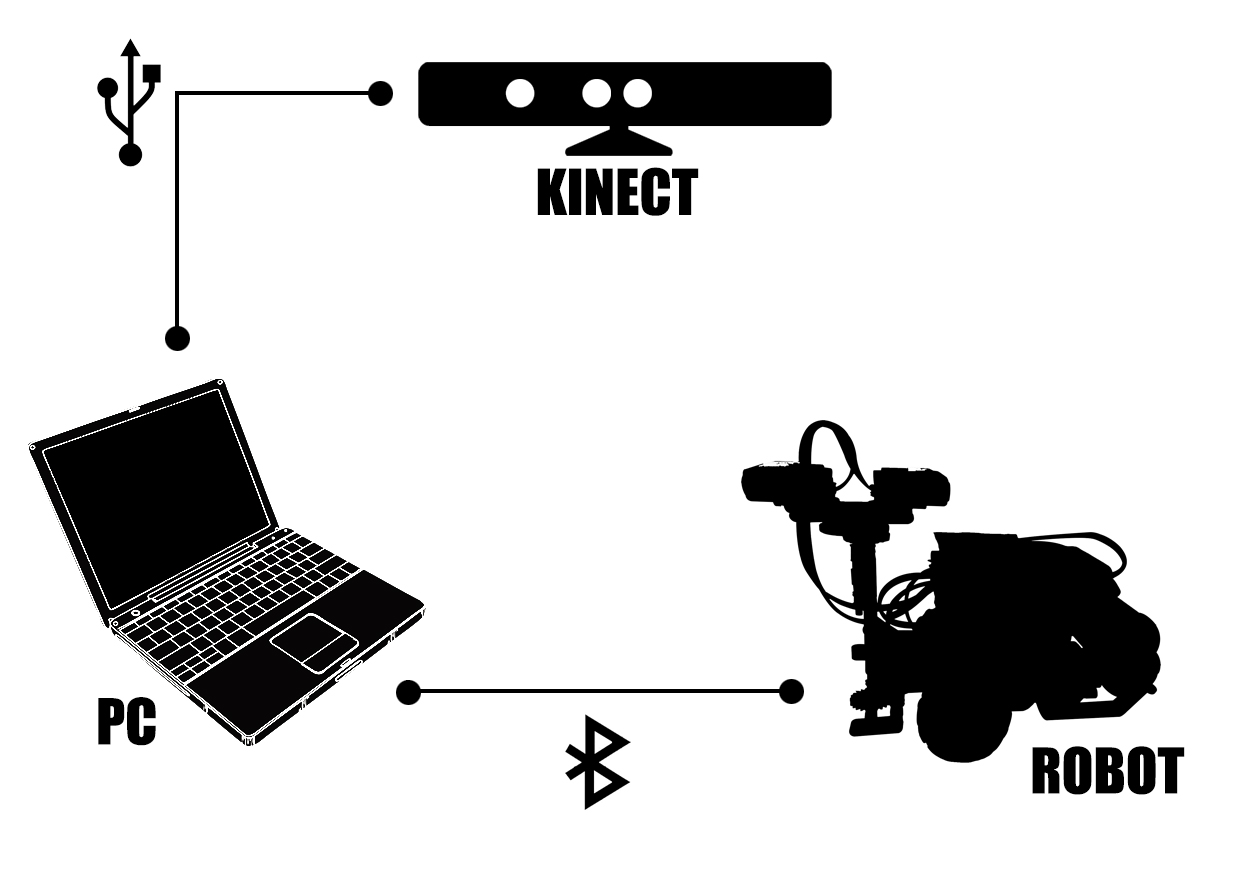
\includegraphics[width=\textwidth]{enheder}
\end{column}
\end{columns}
\end{frame}

\subsection{NXT (Robot)}

\begin{frame}{NXT Software}
Vigtigste filer og deres funktionalitet:
\begin{description}
\item[MainTask.nxc]{Main task/loop og kommunikation fra PC}
\item[Communication.nxc]{Kommunikation til PC}
\item[Navigation.nxc]{Navigation i verden}
\item[Sensor.nxc]{Observation af verden}
\item[MCTasks.nxc]{Motor Control; til bedre styring af motorer}
\end{description}
\end{frame}

\subsection{PC}

\begin{frame}{PC Software}
\begin{center}
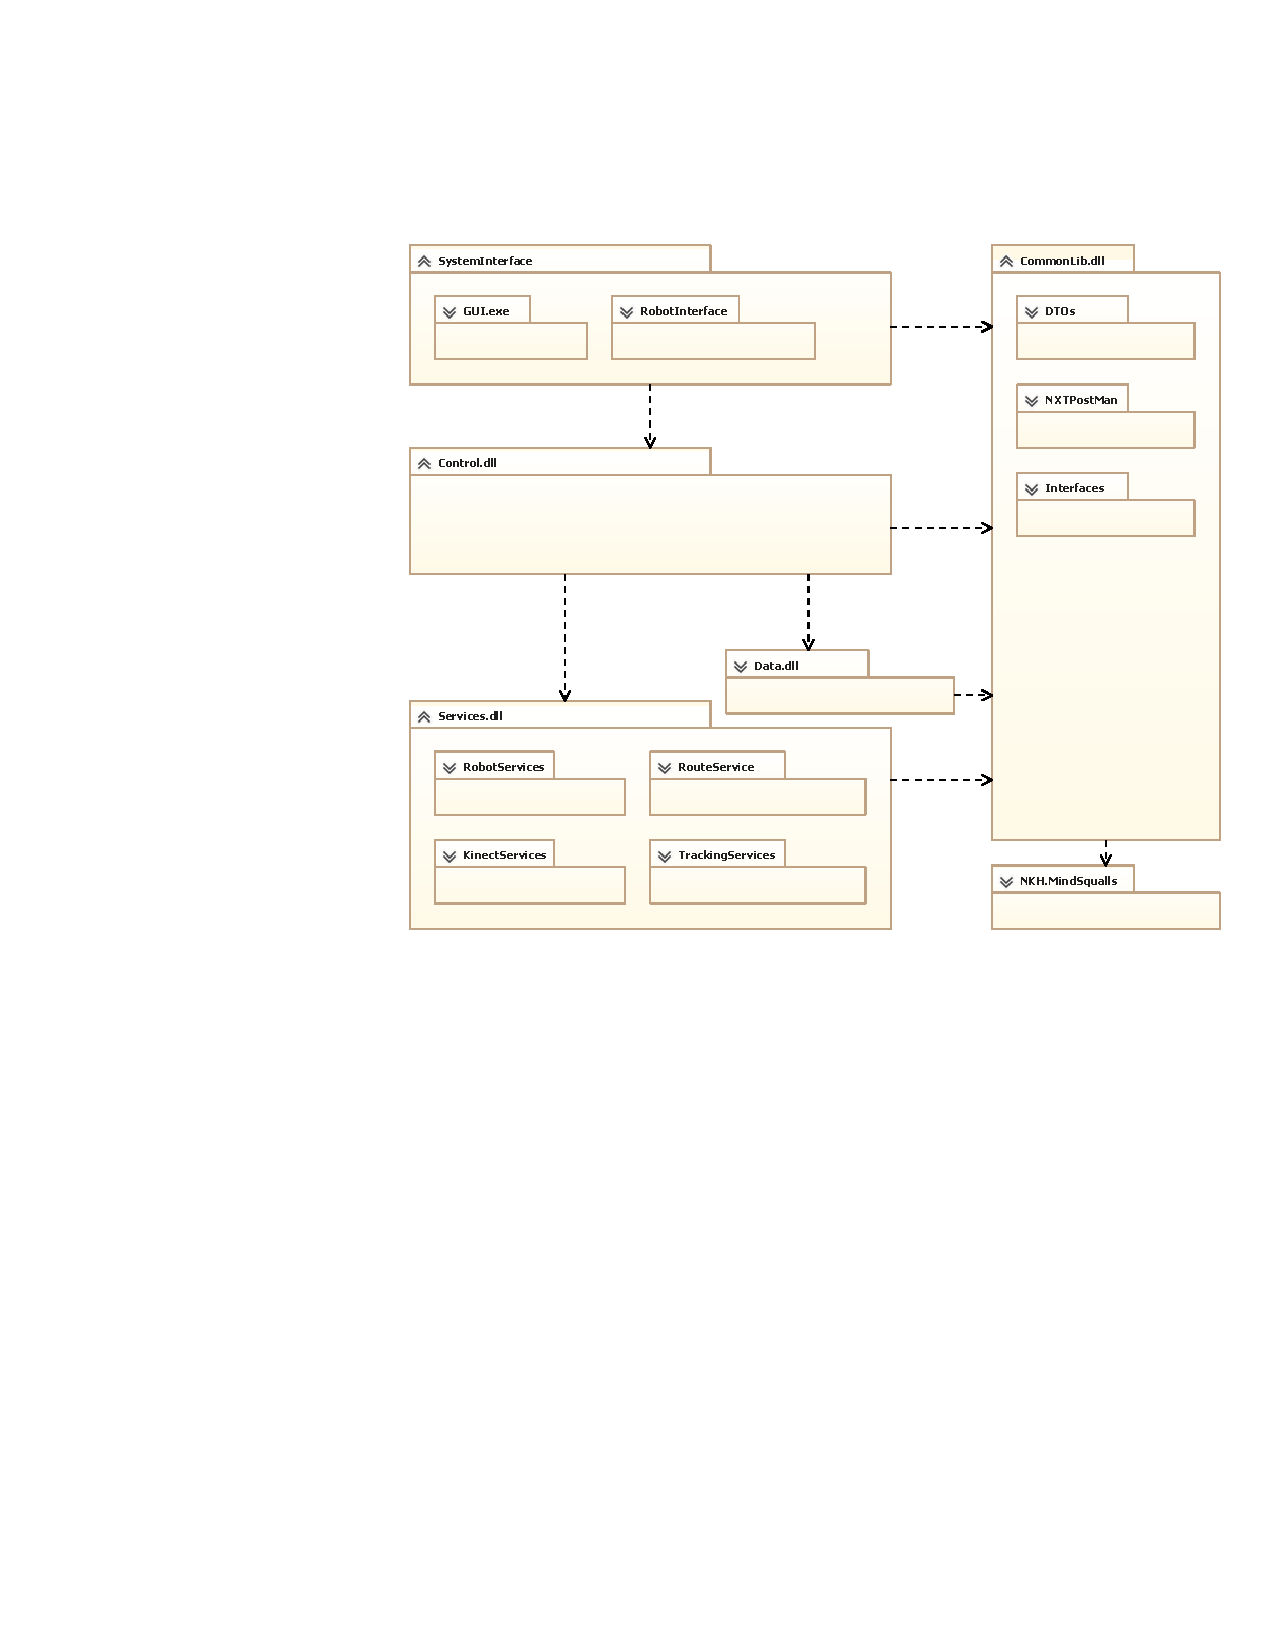
\includegraphics[height=.9\textheight]{arkitektur/namespaces}
\end{center}
\end{frame}

\subsection{Kommunikation}

\begin{frame}{Protokol}
\begin{description}
\item[Generelt]{$< BeskedType >< Indhold >$}
\item[Eksempel]{Robot anmoder om lokation\\
\texttt{0}\\
PC sender lokation\\
\texttt{\textcolor{red}{52}-0213.5\textcolor{red}{00126.9}00187.4}}
\end{description}
\end{frame}

\begin{frame}{Flow}
Tilstandssekvensdiagram? Komponentdiagram? Vigtigt/spændende?
\end{frame}
